% !TEX program = pdflatex
% 第十四次固体物理作业
\documentclass[UTF8,10pt,a4paper]{article}
\usepackage{ctex}
% \catcode`\。=\active
% \newcommand{。}{.}
\newcommand{\CourseName}{固体物理}
\newcommand{\CourseCode}{PHYS1502}
\newcommand{\Semester}{2019-2020学年第二学期}
\newcommand{\ProjectName}{第十四次作业}
\newcommand{\DueTimeType}{截止时间}
\newcommand{\DueTime}{2020. 6. 12(周五)17:00}
\newcommand{\StudentName}{陈稼霖}
\newcommand{\StudentID}{45875852}
\usepackage[vmargin=1in,hmargin=.5in]{geometry}
\usepackage{fancyhdr}
\usepackage{lastpage}
\usepackage{calc}
\pagestyle{fancy}
\fancyhf{}
\fancyhead[L]{\CourseName}
\fancyhead[C]{\ProjectName}
\fancyhead[R]{\StudentName}
\fancyfoot[R]{\thepage\ / \pageref{LastPage}}
\setlength\headheight{12pt}
\fancypagestyle{FirstPageStyle}{
    \fancyhf{}
    \fancyhead[L]{\CourseName\\
        \CourseCode\\
        \Semester}
    \fancyhead[C]{{\Huge\bfseries\ProjectName}\\
        \DueTimeType\ : \DueTime}
    \fancyhead[R]{姓名 : \makebox[\widthof{\StudentID}][s]{\StudentName}\\
        学号 : \StudentID\\
        成绩 : \underline{\makebox[\widthof{\StudentID}]{}}}
    \fancyfoot[R]{\thepage\ / \pageref{LastPage}}
    \setlength\headheight{36pt}
}
\usepackage{amsmath,amssymb,amsthm,bm}
\allowdisplaybreaks[4]
\newtheoremstyle{Problem}
{}
{}
{}
{}
{\bfseries}
{.}
{ }
{第\thmnumber{ #2}\thmname{ #1}\thmnote{ (#3)} 得分: \underline{\qquad\qquad}}
\theoremstyle{Problem}
\newtheorem{prob}{题}
\newtheoremstyle{Solution}
{}
{}
{}
{}
{\bfseries}
{:}
{ }
{\thmname{#1}}
\makeatletter
\def\@endtheorem{\qed\endtrivlist\@endpefalse}
\makeatother
\theoremstyle{Solution}
\newtheorem*{sol}{解}
\providecommand{\abs}[1]{\left\lvert#1\right\rvert}
\usepackage{graphicx}
\usepackage{ulem}
\begin{document}
\thispagestyle{FirstPageStyle}
\begin{prob}[(19.4)$\ddagger$ Para and Diamagnetism]
    Manganese (Mn, atomic number $=25$) forms an atomic vapor at $2000$ K with vapor pressure $10^5$ Pa. You can consider this vapor to be an ideal gas.
    \begin{enumerate}
        \item[(a)] Determine $L$, $S$, and $J$ for an isolated manganese atom. Determine the paramagnetic contribution to the (Cuire) susceptibility of this gas at $2000$ K.
        \item[(b)] In addition to the Cuire susceptibility, the manganese atom will also have some diamagnetic susceptibility due to its filled core orbitals. Determine the Larmor Diamagnetism of the gas at $2000$ K. You may assume the atomic radius of an Mn atom is one Angstrom.\\
            Make sure you know the derivations of all the formulas you use!
    \end{enumerate}
\end{prob}
\begin{sol}
    \begin{enumerate}
        \item[(a)] 锰原子的壳层结构为[Ar]4s$^2$3d$^5$,其最外层的3d轨道恰好半满,故$L=0$,$S=\frac{5}{2}$,$J=L+S=\frac{5}{2}$. 锰原子在外加磁场方向的总角动量投影分量$m_J$可以取为$-\frac{5}{2},-\frac{3}{2},-\frac{1}{2},\frac{1}{2},\frac{3}{2},\frac{5}{2}$. 其磁矩在外加磁场中的能量为
        \begin{align}
            E=g_Jm_J\mu_BB,\quad J=-\frac{5}{2},-\frac{3}{2},-\frac{1}{2},\frac{1}{2},\frac{3}{2},\frac{5}{2}.
        \end{align}
        由于锰原子的总角动量完全由其电子贡献,故其朗德$g$因子$J_g=2$. 锰蒸汽的配分函数为
        \begin{align}
            Z=\sum_{m_J=-\frac{5}{2}}^{\frac{5}{2}}e^{-\beta g_Jm_J\mu_BB},\quad m_J=-\frac{5}{2},-\frac{3}{2},-\frac{1}{2},\frac{1}{2},\frac{3}{2},\frac{5}{2}.
        \end{align}
        由于我们仅计算磁化率的线性部分(也就是在磁场较小时磁极化强度和磁场强度的比值),故可对上式进行级数展开并取其低阶项
        \begin{align}
            Z=\sum_{m_J=-\frac{5}{2}}^{\frac{5}{2}}\left[1-(\beta g_Jm_J\mu_BB)+\frac{1}{2}(\beta g_Jm_J\mu_BB)^2+\cdots\right]\approx 6+\frac{35}{2}(\beta g_Jm_J\mu_BB)^2.
        \end{align}
        单个锰原子的平均磁矩为
        \begin{align}
            \langle m\rangle=-\frac{\partial F}{\partial B}=-\frac{\partial(-k_BT\ln Z)}{\partial B}=k_BT\frac{\frac{35}{2}(\beta g_J\mu_B)^2B}{6+\frac{35}{4}(\beta g_J\mu_BB)^2}\approx\frac{35}{12}\beta(g_J\mu_B)^2B.
        \end{align}
        锰蒸汽的磁极化率为
        \begin{align}
            \chi=\lim_{H\rightarrow 0}\frac{\partial M}{\partial H}=\lim_{B\rightarrow 0}\frac{\partial(n\langle m\rangle)}{\partial(B/\mu_0)}=\frac{35}{12}n\beta\mu_0(g_J\mu_B)^2.
        \end{align}
        视锰蒸汽为理想气体,则
        \begin{align}
            n=\frac{P}{k_BT}.
        \end{align}
        锰蒸汽的磁极化率为
        \begin{align}
            \chi=\frac{35}{12}\frac{P}{(k_BT)^2}\mu_0(g_J\mu_B)^2=\frac{35}{12}\frac{10^5}{(1.38\times 10^{-23}\times 2000)^2}\times 4\pi\times 10^{-7}\times(2\times 9.27\times 10^{-24})^2=1.65\times 10^{-7}.
        \end{align}
        \item[(b)] 电子在外场中的哈密顿量为
        \begin{align}
            \nonumber H=&\frac{(\bm{p}^2+e\bm{A})^2}{2m}+V(\bm{r})-\bm{m}\cdot\bm{B}\\
            =&\frac{(\bm{p}+e\bm{A})^2}{2m}+V(\bm{r})-g_Jm_J\mu_BB.\\
        \end{align}
        不失一般性,采用具有旋转对称性的规范
        \begin{align}
            \bm{A}=\frac{1}{2}\bm{B}\times\bm{r}.
        \end{align}
        则电子在外场中的哈密顿量可化为
        \begin{align}
            H=&\frac{\bm{p}^2}{2m}+\frac{(\bm{p}\cdot\bm{A}+\bm{A}\cdot\bm{p})}{2m}+\frac{e^2\bm{A}^2}{2m}+V(\bm{r})-g_Jm_J\mu_BB\\
            \nonumber&(\text{因为$\bm{p}$和$\bm{A}$对易})\\
            \nonumber=&\frac{\bm{p}^2}{2m}+\frac{e\bm{p}\cdot(\bm{B}\times\bm{r})}{2m}+\frac{e^2}{2m}\frac{(\bm{B}\times\bm{r})^2}{4}+V(\bm{r})-g_Jm_J\mu_BB,
        \end{align}
        其中第三项$\frac{q^2}{2m}\frac{(\bm{B}\times\bm{r})^2}{4}$即为逆磁项. 假设外加磁场沿着$z$轴,这一项的期望值为
        \begin{align}
            \nonumber\frac{e^2}{8m}\langle(\bm{B}\times\bm{r})^2\rangle=&\frac{q^2B^2}{8m}\langle x^2+y^2\rangle\\
            \nonumber=&\frac{e^2B^2}{8m}\frac{2}{3}\langle x^2+y^2+z^2\rangle\\
            \nonumber=&\frac{e^2B^2}{8m}\frac{2}{3}\langle r^2\rangle\\
            =&\frac{e^2B^2}{12m}\langle r^2\rangle.
        \end{align}
        逆磁项在每个电子上贡献的磁矩为
        \begin{align}
            m=-\frac{\partial\left(\frac{e^2B^2}{12m}\langle r^2\rangle\right)}{\partial B}=-\frac{e^2}{6m}B\langle r^2\rangle,
        \end{align}
        逆磁项贡献的磁极化率为
        \begin{align}
            \chi=\lim_{H\rightarrow 0}\frac{\partial M}{\partial H}=\lim_{B\rightarrow 0}\frac{\partial(\rho m)}{\partial(B/\mu_0)}=-\frac{\mu_0\rho e^2}{6m}\langle r^2\rangle,
        \end{align}
        其中锰原子中有$25$个电子,电子数密度为原子数密度的$25$倍
        \begin{align}
            \rho=25n=\frac{25P}{k_BT}=\frac{25\times 10^5}{1.38\times 10^{-23}\times 2000}\text{m}^{-3}=9.06\times 10^{25}\text{m}^{-3},
        \end{align}
        取$\langle r^2\rangle=10^{-20}\text{m}^2$,计算得到逆磁项贡献的磁极化率为
        \begin{align}
            \chi=-\frac{\mu_0\rho e^2}{6m}\langle r^2\rangle=-\frac{4\pi\times 10^{-7}\times 9.06\times 10^{25}\times(1.60\times 10^{-19})^2}{6\times 9.11\times 10^{-31}}\times 10^{-20}=-5.33\times 10^{-9}.
        \end{align}
    \end{enumerate}
\end{sol}

\begin{prob}[(19.5)$\ddagger$ Diamagnetism]
    \begin{enumerate}
        \item[(a)] Argon is a noble gas with atomic number $18$ and atomic radius of about $.188$ nm. At low temperature it forms an fcc crystal. Estimate the magnetic susceptibility of solid argon.
        \item[(b)] The wavefunction of an electron bound to an impurity in $n$-type silicon is hydrogen in form. Estimate the impurity contribution to the diamagnetic susceptibility of a Si crystal containing $10^{20}~m^{-3}$ donor given that the electron effective mass $m^*=0.4m_e$ and the relative permittivity is $\epsilon_r=12$. How does this value compare to the diamagnetism of the underlying silicon atoms? Si has atomic number $14$, atomic weight $28.09$, and density $2.33~\text{g}/\text{cm}^3$.
    \end{enumerate}
\end{prob}
\begin{sol}
    \begin{enumerate}
        \item[(a)] 因为Ar是惰性元素,其各个壳层都已被电子占满,故其哈密顿的顺磁项总和为零,呈现出抗磁性,其磁极化率为
        \begin{align}
            \chi=-\frac{\mu_0\rho e^2}{6m}\langle r^2\rangle.
        \end{align}
        Ar晶体为fcc晶体,每个晶胞中有$4$个原子,故原子数密度为
        \begin{align}
            n=\frac{4}{(2\sqrt{2}a)^3}=\frac{1}{4\sqrt{2}(0.188\times 10^{-9}\text{m})^3}=2.66\times 10^{28}\text{m}^{-3}.
        \end{align}
        每个Ar原子中有$18$个电子,故电子数密度为
        \begin{align}
            \rho=18n=18\times 2.66\times 10^{28}\text{m}^{-3}=4.79\times 10^{29}\text{m}^{-3}.
        \end{align}
        Ar晶体的磁极化率为
        \begin{align}
            \chi=-\frac{\mu_0\rho e^2}{6m}\langle r^2\rangle=-\frac{4\pi\times 10^{-7}\times 4.79\times 10^{28}\times(1.60\times 10^{-19})^2}{6\times 9.11\times 10^{-31}}\times(0.188\times 10^{-9})^2\text{m}^{-3}=9.96\times 10^{-5}.
        \end{align}
        \item[(b)] 将施主原子视为类氢原子,其玻尔半径为
        \begin{align}
            a_0=\frac{4\pi\epsilon_0\epsilon_r\hbar^2}{m^*e^2}=\frac{4\pi\epsilon_0\epsilon_r\hbar^2}{0.4m_ee^2}=\frac{4\pi\times 8.85\times 10^{-12}\times 12\times(6.63\times 10^{-34}/2\pi)^2}{0.4\times 9.11\times 10^{-31}\times(1.60\times 10^{-19})^2}\text{m}=1.59\times 10^{-9}\text{m}.
        \end{align}
        施主原子贡献的磁极化率为
        \begin{align}
            \chi_{donor}=-\mu_0\frac{\rho_{donor}e^2}{6m^*}a_0^2=-4\pi\times 10^{-7}\times\frac{10^{20}Z_{donor}\times(1.60\times 10^{-19})^2}{6\times 0.4\times 9.11\times 10^{-31}}\times(1.59\times 10^{-9})^2Z_{donor}=-3.72\times 10^{-12}Z_{donor},
        \end{align}
        其中$Z_{donor}$是每个施主原子的原子序数(即所带的电子数).\\
        Si的原子数密度为
        \begin{align}
            n_{Si}=\frac{2.33\times 10^3\text{kg}/\text{m}^{-3}}{28.09\times 10^{-3}\text{kg}\cdot\text{mol}^{-1}/6.02\times 10^{23}\text{mol}^{-1}}=4.99\times 10^{28}\text{m}^{-3}.
        \end{align}
        Si的原子序数为$14$,故Si的电子数密度为
        \begin{align}
            \rho_{Si}=14n_{Si}=6.99\times 10^{29}\text{m}^{-3}.
        \end{align}
        Si的传统晶胞中有$8$个原子,故其传统晶胞的体积为$a^3=\frac{8}{n_{Si}}$,两个最近的Si原子的距离为$\frac{\sqrt{3}}{4}a$,故Si原子半径为
        \begin{align}
            r_{Si}=\frac{1}{2}\frac{\sqrt{3}}{4}\left(\frac{8}{n_{Si}}\right)^{1/3}=1.18\times 10^{-10}\text{m}.
        \end{align}
        Si晶体的磁极化率为
        \begin{align}
            \chi_{Si}=-\mu_0\frac{\rho_{Si}e^2}{6m}r_{Si}^2=-4\pi\times 10^{-7}\times\frac{6.99\times 10^{29}\times(1.60\times 10^{-19})^2}{6\times 9.11\times 10^{-31}}\times(1.18\times 10^{-10})^2=-5.73\times 10^{-5},
        \end{align}
        远远大于施主原子贡献的磁极化率.
    \end{enumerate}
\end{sol}

\begin{prob}[(19.6) Paramagnetism]
    Consider a gas of monoatomic atoms with spin $S=1/2$ (and $L=0$) in a magnetic field $B$. The gas has density $n$.
    \begin{enumerate}
        \item[(a)] Calculate the magnetization as a function of $B$ and $T$. Determine the susceptibility.
        \item[(b)] Calculate the contribution to the specific heat of this gas due to the spins. Sketch this contribution as a function of $\mu_BB/k_BT$.
    \end{enumerate}
\end{prob}
\begin{sol}
    \begin{enumerate}
        \item[(a)] 因为气体原子仅有自旋量子数$S=\frac{1}{2}$,而轨道量子数$L=0$,故$L=\frac{1}{2}$,其总角动量在外加磁场方向的投影分量$m_J=-\frac{1}{2},\frac{1}{2}$. 且由于总角动量完全由电子自旋贡献,故朗德$g$因子$g=2$. 单个气体原子的磁矩在外加磁场$B$中的能量为
        \begin{align}
            E=-g_Jm_J\mu_BB,\quad m_J=\pm\frac{1}{2}.
        \end{align}
        体系的配分函数为
        \begin{align}
            Z=\sum_{m_J=\pm\frac{1}{2}}e^{-\beta E}=e^{-\beta\mu_BB}+e^{\beta\mu_BB}.
        \end{align}
        自由能为
        \begin{align}
            F=-k_BT\ln Z.
        \end{align}
        单个原子的磁矩的期望值为
        \begin{align}
            \langle m\rangle=-\frac{\partial F}{\partial B}=\mu_B\tanh(\beta\mu_BB).
        \end{align}
        气体的磁极化率为
        \begin{align}
            \chi=\lim_{H\rightarrow 0}\frac{\partial M}{\partial H}=\lim_{B\rightarrow 0}\frac{\partial(nm)}{\partial(B/\mu_0)}=\mu_0n\mu_B^2\beta.
        \end{align}
        \item[(b)] \uline{每个}自旋贡献的能量为
        \begin{align}
            U=-\frac{\partial\ln Z}{\partial\beta}=-\mu_BB\tanh(\beta\mu_BB).
        \end{align}
        \uline{每个}自旋贡献的热容为
        \begin{align}
            C=\frac{\partial U}{\partial T}=\frac{1}{k_BT^2}(\mu_BB)^2\text{sech}^2(\beta\mu_BB)=k_B(\beta\mu_BB)^2\text{sech}^2(\beta\mu_BB).
        \end{align}
        热容$C$作为关于$\frac{\mu_BB}{k_BT}$的函数的曲线如图\ref{3-C}.
        \begin{figure}[h]
            \centering
            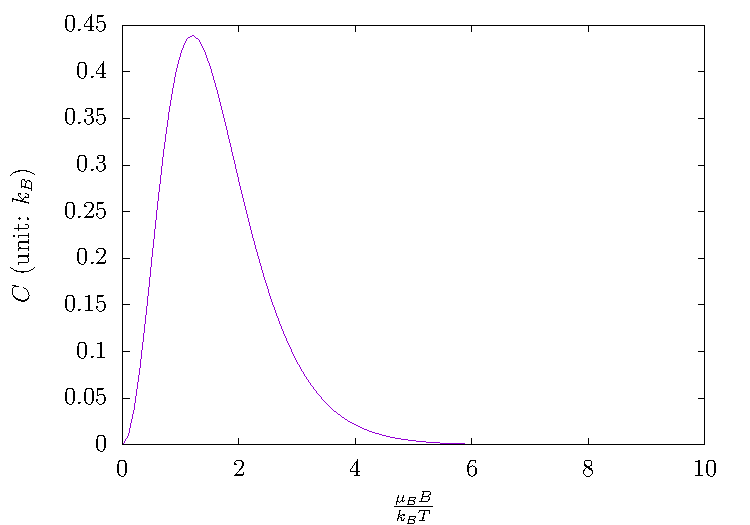
\includegraphics[width=.5\textwidth]{3-C.pdf}
            \caption{热容$C$作为关于$\frac{\mu_BB}{k_BT}$的函数的曲线}
            \label{3-C}
        \end{figure}
    \end{enumerate}
\end{sol}

\begin{prob}[(20.1)$\ddagger$ Ferromagnetic vs Antiferromagnetic States]
    Consider the Heisenberg Hamiltonian
    \[
        \mathcal{H}=-\frac{1}{2}\sum_{\langle i,j\rangle}J\bm{S}_i\cdot\bm{S}_j+\sum_ig\mu_{B}\bm{B}\cdot\bm{S}_i.\tag{20.6}
    \]
    \begin{enumerate}
        \item[(a)] For $J>0$, i.e., for the case of a ferromagnet, intuition tells us that the ground state of this Hamiltonian should simply have all spins aligned. Consider such a state. Show that this is an eigenstate of the Hamiltonian Eq. 20.6 and find its energy.
        \item[(b)] For $J<0$, the case of an antiferromagnet on a cubic lattice on a cubic lattice, one might expect that (at least for $\bm{B}=0$) the state where spins on alternating sites point in opposite directions might be an eigenstate. Unfortunately, this is not precisely true. Consider such a state of the system. Show that the state in question is not an eigenstate of the Hamiltonian.\\
        Although the intuition of alternating spins on alternating site is not perfect, it becomes reasonable for systems with large spins $S$. For smaller spins (like spin $1/2$) one needs to consider so-called "quantum fluctuations" (which is much more advanced, so we will not to do that here).
    \end{enumerate}
\end{prob}
\begin{sol}
    \begin{enumerate}
        \item[(a)] 将内积$\bm{S}_i\cdot\bm{S}_j$表示为
        \begin{align}
            \bm{S}_i\cdot\bm{S}_j=\frac{1}{2}(S_i^+S_j^-+S_i^-S_j^+)+S_i^zS_j^z,
        \end{align}
        其中升算符
        \begin{align}
            S_i^+=S_i^x+iS_i^y,
        \end{align}
        降算符
        \begin{align}
            S_i^-=S_i^x-iS_i^y,
        \end{align}
        它们作用在自旋态上的效果是
        \begin{align}
            S_i^+\lvert\uparrow_i\rangle=&0,\\
            S_i^+\lvert\downarrow_i\rangle=&2S\lvert\uparrow_i\rangle,\\
            S_i^-\lvert\uparrow_i\rangle=&2S\lvert\downarrow_i\rangle\\
            S_i^-\lvert\downarrow_i\rangle=&0,\\
            S_i^z\lvert\uparrow_i\rangle=&S\lvert\uparrow_i\rangle,\\
            S_i^z\lvert\downarrow_i\rangle=&-S\lvert\downarrow_i\rangle,
        \end{align}
        故
        \begin{align}
            \bm{S}_i\bm{S}_j\lvert\uparrow_i\uparrow_j\rangle=\left[\frac{1}{2}(S_i^+S_j^-+S_i^-S_j^+)+S_i^zS_j^z\right]\lvert\uparrow_i\uparrow_j\rangle=S^2\lvert\uparrow_i\uparrow_j\rangle,
        \end{align}
        对于铁磁性材料,其中所有自旋同向,体系的总状态为
        \begin{align}
            \lvert\psi\rangle=\prod_{i}\otimes\lvert\uparrow_i\rangle.
        \end{align}
        将哈密顿作用在这一状态上得
        \begin{align}
            \nonumber\mathcal{H}\lvert\psi\rangle=&\left[-\frac{1}{2}\sum_{\langle i,j\rangle}J\bm{S}_i\cdot\bm{S}_j+\sum_ig\mu_B\bm{B}\cdot\bm{S}_i\right]\prod_i\otimes\lvert\uparrow_i\rangle\\
            \nonumber=&-\frac{1}{2}\sum_iJzS^2\prod_i\otimes\lvert\uparrow_i\rangle+\sum_ig\mu_BBS\prod_i\otimes\lvert\uparrow_i\rangle\\
            =&(-JzS^2/2-NgS\mu_BB)\lvert\psi\rangle.
        \end{align}
        其中$z$是每个自旋周围的相邻自旋数,故所有自旋同向排列是这一哈密顿量的本征态,它对应的本征能量为
        \begin{align}
            E=-JzS^2/2-NgS\mu_BB.
        \end{align}
        \item[(b)] 简单起见,我们可以直接看只有两个自旋的系统,此时所谓的相邻自旋反向的状态为
        \begin{align}
            \lvert\psi\rangle=\lvert\uparrow_1\downarrow_2\rangle.
        \end{align}
        将$\bm{B}\cdot\bm{S}$作用在这一状态上,有
        \begin{align}
            \bm{B}\cdot\bm{S}\lvert\uparrow_1\downarrow_2\rangle=BS\lvert\uparrow_1\downarrow_2\rangle,
        \end{align}
        没有什么问题,但若将$\bm{S}_1\cdot\bm{S}_2$作用在这一状态上,则
        \begin{align}
            \bm{S}_1\cdot\bm{S}_2\lvert\uparrow_1\downarrow_2\rangle=\left[\frac{1}{2}(S_1^+S_2^-+S_1^-S_2^+)+S_1^zS_2^z\right]\lvert\uparrow_1\downarrow_2\rangle=S^2\left[\frac{1}{2}\lvert\downarrow_1\uparrow_2\rangle+\lvert\uparrow_1\downarrow_2\rangle\right],
        \end{align}
        显然,这样的相邻自旋相反的状态无法成为该哈密顿量的本征态.
    \end{enumerate}
\end{sol}

\begin{prob}[(20.2) Frustation]
    Consider the Heisenberg Hamiltonian as in Exercise 20.1 with $J<0$, and treat the spins as classical vectors.
    \begin{enumerate}
        \item[(a)] If the system consist of only three spins arranged in a triangle (as in Fig. 20.2), show that the ground state has each spin oriented $120^{\circ}$ from its neighbor.
        \item[(b)] For an infinite triangle lattice, what does the ground state look like?
    \end{enumerate}
    \begin{figure}[h]
        \centering
        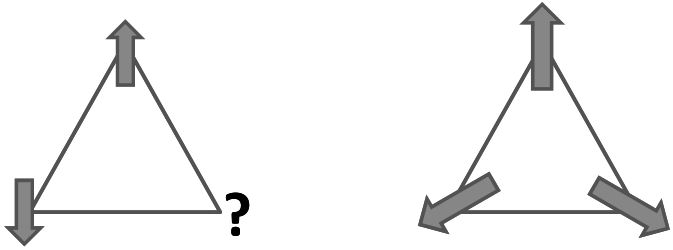
\includegraphics[width=.5\textwidth]{5.png}
        \caption{Fig 20.2}
    \end{figure}
\end{prob}
\begin{sol}
    (假设这三个自旋都具有相同的$S$)
    \begin{enumerate}
        \item[(a)] 体系的哈密顿量为
        \begin{align}
            \nonumber\mathcal{H}=&J(\bm{S}_1\cdot\bm{S}_2+\bm{S}_2\cdot\bm{S}_3+\bm{S})\\
            \nonumber=&\frac{J}{2}[(\bm{S}_1+\bm{S}_2+\bm{S}_3)^2-(\bm{S}_1\cdot\bm{S}_1+\bm{S}_2\cdot\bm{S}_3+\bm{S}_3\cdot\bm{S}_3)]\\
            =&\frac{J}{2}[(\bm{S}_1+\bm{S}_2+\bm{S}_3)^2-3S^2].
        \end{align}
        故要使得体系能量最小,需要
        \begin{align}
            \bm{S}_1+\bm{S}_2+\bm{S}_3=0,
        \end{align}
        也就对应着三个自旋相互之间呈$120^{\circ}$夹角的情形.
        \item[(b)] 对于具有无限个自旋的三角晶格,其哈密顿量实际上就是无数个上一小题中哈密顿量的加和,我们只要使得晶格中每个小三角形中的三个自旋之间夹角互为$120^{\circ}$(如图\ref{5-InfiniteTriangleLattice}),即可使使这总哈密顿量最小.
        \begin{figure}[h]
            \centering
            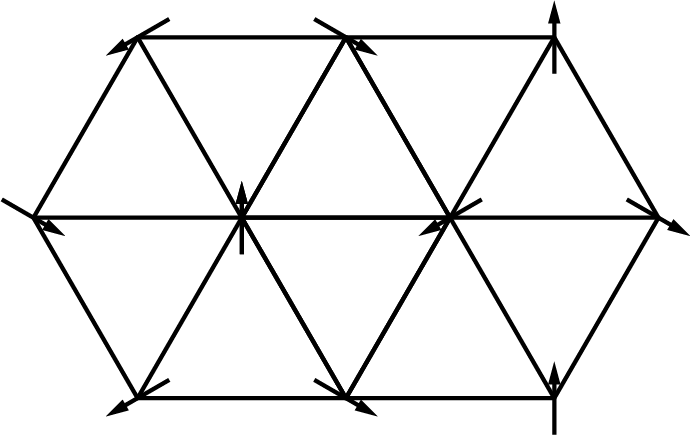
\includegraphics[width=.5\textwidth]{5-InfiniteTriangleLattice.png}
            \caption{无限个自旋的三角晶格的能量最低的状态}
            \label{5-InfiniteTriangleLattice}
        \end{figure}
    \end{enumerate}
\end{sol}

\begin{prob}[(20.4) Small Heisenberg Models]
    \begin{enumerate}
        \item[(a)] Consider a Heisenberg model containing a chain of two spins, so that
        \[
            \mathcal{H}=-J\bm{S}_1\cdot\bm{S}_2.
        \]
        Supposing these spins have $S=1/2$, calculate the energy spectrum of this system. Hint: Write $2\bm{S}_1\cdot\bm{S}_2=(\bm{S}_1+\bm{S}_2)^2-\bm{S}_1^2-\bm{S}_2^2$.
        \item[(b)] Now consider three spins forming a triangle (as shown in Fig. 20.2). Again assuming these spins are $S=1/2$, calculate the spectrum of the system. Hint: Use the same trick as in part (a)!
        \item[(c)] Now consider three spins forming a triangle (as shown in Fig. 20.2). Again assuming these spins are $S=1/2$, calculate the spectrum of the system.
    \end{enumerate}
\end{prob}
\begin{sol}
    \begin{enumerate}
        \item[(a)] 系统哈密顿可写为
        \begin{align}
            \mathcal{H}=-\frac{J}{2}[(\bm{S}_1+\bm{S}_2)^2-\bm{S}_1^2-\bm{S}_2^2].
        \end{align}
        该哈密顿的矩阵元为
        \begin{align}
            \langle\uparrow_1\uparrow_2\rvert\mathcal{H}\lvert\uparrow_1\uparrow_2\rangle=\langle\downarrow_1\downarrow_2\rvert\mathcal{H}\lvert\downarrow_1\downarrow_2\rangle=-\frac{J}{2}\left[1(1+1)-\frac{1}{2}\left(\frac{1}{2}+1\right)-\frac{1}{2}\left(\frac{1}{2}+1\right)\right]=&-\frac{J}{4},\\
            \langle\uparrow_1\downarrow_2\rvert\mathcal{H}\lvert\uparrow_1\downarrow_2\rangle=\langle\downarrow_1\uparrow_2\rvert\mathcal{H}\lvert\downarrow_1\uparrow_2\rangle=-\frac{J}{2}\left[0(0+1)-\frac{1}{2}\left(\frac{1}{2}+1\right)-\frac{1}{2}\left(\frac{1}{2}+1\right)\right]=&\frac{3J}{4},\\
        \end{align}
        其余矩阵元为$0$,哈密顿矩阵为
        \begin{align}
            H=J\left(\begin{matrix}
                -\frac{1}{4}&0&0&0\\
                0&\frac{3}{4}&0&0\\
                0&0&\frac{3}{4}&0\\
                0&0&0&-\frac{1}{4}
            \end{matrix}\right).
        \end{align}
        系统的本征能量即为其对角元:
        \begin{align}
            E=-\frac{J}{4},\frac{3J}{4},\frac{3J}{4},-\frac{J}{4}.
        \end{align}
        \item[(b)] 对于具有三个自旋的体系,其哈密顿可写为
        \begin{align}
            \mathcal{H}=-\frac{J}{2}[(\bm{S}_1+\bm{S}_2+\bm{S}_3)^2-\bm{S}_1^2-\bm{S}_2^2-\bm{S}_3^2].
        \end{align}
        该哈密顿的矩阵元为
        \begin{align}
            &\langle\uparrow_1\uparrow_2\uparrow_3\rvert\mathcal{H}\lvert\uparrow_1\uparrow_2\uparrow_3\rangle=\langle\downarrow_1\downarrow_2\downarrow_3\rvert\mathcal{H}\lvert\downarrow_1\downarrow_2\downarrow_3\rangle=-\frac{J}{2}\left[\frac{3}{2}\left(\frac{3}{2}+1\right)-\frac{1}{2}\left(\frac{1}{2}+1\right)-\frac{1}{2}\left(\frac{1}{2}+1\right)-\frac{1}{2}\left(\frac{1}{2}+1\right)\right]=-\frac{3}{4}J,\\
            \nonumber&\langle\text{两个自旋朝上,一个自旋朝下}\rvert\mathcal{H}\lvert\text{两个自旋朝上,一个自旋朝下}\rangle\\
            \nonumber=&\langle\text{两个自旋朝下,一个自旋朝上}\rvert\mathcal{H}\lvert\text{两个自旋朝下,一个自旋朝上}\rangle\\
            =&-\frac{J}{2}\left[\frac{1}{2}\left(\frac{1}{2}+1\right)-\frac{1}{2}\left(\frac{1}{2}+1\right)-\frac{1}{2}\left(\frac{1}{2}+1\right)-\frac{1}{2}\left(\frac{1}{2}+1\right)\right]=\frac{3}{4}J,\\
        \end{align}
        除此之外的非对角元均为$0$,故系统的本征能量为
        \begin{align}
            E=-\frac{3J}{4},-\frac{3J}{4},\frac{3J}{4},\frac{3J}{4},\frac{3J}{4},\frac{3J}{4},\frac{3J}{4},\frac{3J}{4}.
        \end{align}
        \item[(c)] 对于具有四个自旋的体系,其哈密顿可写为
        \begin{align}
            \mathcal{H}=-\frac{J}{2}[(\bm{S}_1+\bm{S}_2+\bm{S}_3+\bm{S}_4)^2-\bm{S}_1^2-\bm{S}_2^2-\bm{S}_3^2-\bm{S}_4^2].
        \end{align}
        对于四个自旋全部同向的情况,本征能量为
        \begin{align}
            E=-\frac{J}{2}\left[2(2+1)-\frac{1}{2}\left(\frac{1}{2}+1\right)-\frac{1}{2}\left(\frac{1}{2}+1\right)-\frac{1}{2}\left(\frac{1}{2}+1\right)-\frac{1}{2}\left(\frac{1}{2}+1\right)\right]=-\frac{3J}{2}.
        \end{align}
        对于两个自旋朝上,另外两个自旋朝下的情况,本征能量为
        \begin{align}
            E=-\frac{J}{2}\left[0(0+1)-\frac{1}{2}\left(\frac{1}{2}+1\right)-\frac{1}{2}\left(\frac{1}{2}+1\right)-\frac{1}{2}\left(\frac{1}{2}+1\right)-\frac{1}{2}\left(\frac{1}{2}+1\right)\right]=\frac{3J}{2}.
        \end{align}
        对于一个自旋与另外三个自旋反向的情况,本征能量为
        \begin{align}
            E=-\frac{J}{2}\left[1(1+1)-\frac{1}{2}\left(\frac{1}{2}+1\right)-\frac{1}{2}\left(\frac{1}{2}+1\right)-\frac{1}{2}\left(\frac{1}{2}+1\right)-\frac{1}{2}\left(\frac{1}{2}+1\right)\right]=\frac{J}{2}.
        \end{align}
        故系统的本征能谱为
        \begin{align}
            E=-\frac{3J}{2},-\frac{3J}{2},\frac{3J}{2},\frac{3J}{2},\frac{3J}{2},\frac{3J}{2},\frac{3J}{2},\frac{3J}{2},-\frac{J}{2},-\frac{J}{2},-\frac{J}{2},-\frac{J}{2},-\frac{J}{2},-\frac{J}{2},-\frac{J}{2},-\frac{J}{2}.
        \end{align}
    \end{enumerate}
\end{sol}

\begin{prob}[(20.5) One-Dimensional Ising Model with $B=0$]
    \begin{enumerate}
        \item[(a)] Consider the one-dimensional Ising model with spin $S=1$. We write the Hamiltonian for a chain of $N$ spins in zero magnetic field as
        \[
            \mathcal{H}=-J\sum_{i=1}^{N-1}\sigma_i\sigma_{i+1}
        \]
        where each $\sigma_i$ takes the value $\pm 1$. The partition function can be written as
        \[
            Z=\sum_{\sigma_1,\sigma_2,\cdots,\sigma_N}e^{-\beta H}.
        \]
    Using the transformation $R_i=\sigma_i\sigma_{i+1}$ rewrite the partition function as a sum over the $R$ variables, and hence evaluate the partition function.
    \begin{itemize}
        \item[$\triangleright$] Show that the free energy has cusp or discontinuity at any temperature, and hence conclude that there is no phase transition in the one-dimensional Ising model.
    \end{itemize}
    \item[(b)$^*$] At a given temperature $T$, calculate an expression for the probability that $M$ consecutive spins will be pointing in the same direction. How does this probability decay with $M$ for large $M$? What happens as $T$ becomes small? You may assume $N\gg M$.
    \end{enumerate}
\end{prob}
\begin{sol}
    \begin{enumerate}
        \item[(a)] 将哈密顿用$R_i=\sigma_i\sigma_{i+1}$表示
        \begin{align}
            \mathcal{H}=-J\sum_{i=1}^{N-1}R_i
        \end{align}
        设
        \begin{align}
            R=\sum_{i=1}^{N-1}R_i
        \end{align}
        系统的配分函数是每个自旋的子配分函数的乘积,将它也用$R_i=\sigma_i\sigma_{i+1}$表示
        \begin{align}
            Z=\sum_{R=-N+1,-N+3,\cdots,N-1}\left(\begin{matrix}
                N-1\\
                N-1-\abs{R}
            \end{matrix}\right)e^{-\beta JR}=2\left[e^{-\beta J}+e^{\beta J}\right]^{N-1}=2^N\cosh^{N-1}(\beta J).
        \end{align}
        \begin{itemize}
            \item[$\triangleright$] 系统的自由能为
            \begin{align}
                F=-k_BT\ln Z=-k_BTN\ln 2-k_BT(N-1)\ln\cosh(\beta J)\approx-k_BTN\ln 2-k_BTN\ln\cosh(\beta J).
            \end{align}
            自由能关于温度的导数为
            \begin{align}
                \frac{\partial F}{\partial T}=-k_BN\ln 2-k_BN\ln\cosh(\beta J)-N\tanh(\beta T)\frac{J}{T}.
            \end{align}
            无论是自由能还是其导数在$T>0$都是连续的.
        \end{itemize}
        \item[(b)] 与答案有所不同,这里计算的是\textbf{有且仅有}$M$个连续自旋朝同一个方向. 有且仅有$M$个连续自旋朝同一个方向,意味着有$M-1$个$R_i=1$,每个$R_i=+1$的概率为
        \begin{align}
            P(R_i=+1)=\frac{e^{\beta J}}{e^{\beta J}+e^{-\beta J}}.
        \end{align}
        若是有且仅有$M$个自旋朝同一方向,同时意味着其余的自旋相邻反向,这意味着其余$N-M$个$R_i=-1$,每个$R=-1$的概率为
        \begin{align}
            P(R_i=-1)=\frac{e^{-\beta J}}{e^{\beta J}+e^{-\beta J}}.
        \end{align}
        这$M-1$个$R=+1$可以有$N-M+1$种取法,从而有且仅有$M$个连续自旋朝向同一个方向的总概率为
        \begin{align}
            P=(N-1-M)P(R_i=+1)^{M-1}P(R_i=-1)^{N-M}=(N-1-M)\frac{e^{(2M-N+1)\beta J}}{(e^{\beta J}+e^{-\beta J})^{N-1}}.
        \end{align}
        由于$N\gg M$,
        \begin{align}
            P\approx N\frac{e^{(2M-N+1)\beta J}}{(e^{\beta J}+e^{-\beta J})^{N-1}}.
        \end{align}
        当$M$很大时,这一概率随着$M$的减小呈指数衰减;当$T$很小,则
        \begin{align}
            P\approx Ne^{(2M-2N+2)\beta J},
        \end{align}
        这一衰减的趋势更接近于指数衰减.
    \end{enumerate}
\end{sol}
\end{document}